%!TEX program = lualatex
%%_requires compilation with XeLaTeX or LuaLaTeX
\documentclass[10pt,xcolor={table,dvipsnames},t]{beamer}
%%══════════════════════════════════════════════════════════════
%% PRESENTATION SETTINGS
%%══════════════════════════════════════════════════════════════
\usepackage[overridenote]{pdfpc}
%\usepackage[overridenote,hidenotes]{pdfpc}
% "overridenote" must be specified as a package option
\pdfpcsetup{
    % Other settings can be package options, or can go here
    duration=30,
    lastminutes=2,
}

% ============================================================
% LANGUAGE
% ============================================================
% Italiano
%\usepackage[italian]{babel}
%\usepackage[autostyle, italian=guillemets]{csquotes}
% Inglese
\usepackage[british]{babel}
\usepackage[autostyle]{csquotes}

%%══════════════════════════════════════════════════════════════
%% THEME & COLORS
%%══════════════════════════════════════════════════════════════
\usetheme{SNSPisa}  % Template Unipi

%%══════════════════════════════════════════════════════════════
%% GRAPHICS & IMAGES
%%══════════════════════════════════════════════════════════════
\usepackage{tikz}
\usetikzlibrary{
    positioning,      % posizionamento relativo nodi
    arrows.meta,      % frecce moderne
    shapes.geometric, % forme geometriche
    fit               % creare nodi che racchiudono altri nodi
}
\usepackage{svg}
\usepackage{pgfplots}
\usepackage{pgfplotstable}
\usepgfplotslibrary{groupplots}  % grafici multipli in griglia
\pgfplotsset{compat=1.18}        % versione più recente stabile

%%══════════════════════════════════════════════════════════════
%% MATHEMATICS
%%══════════════════════════════════════════════════════════════
\usepackage{amsmath}  % equazioni matematiche avanzate
\usepackage{amssymb}  % simboli matematici aggiuntivi
\usepackage{proof}    % inference rules
\usepackage{bussproofs}
\usepackage{stmaryrd} % semantics brackets
\usepackage{mathrsfs}

%%══════════════════════════════════════════════════════════════
%% CODE LISTINGS
%%══════════════════════════════════════════════════════════════
\usepackage{listings}      % presentazione codice sorgente
\lstset{
  escapeinside={(*@}{@*)}
}
\usepackage{lstautogobble} % rimuove l'indentazione automatica del codice
\usepackage{llvmlisting}   % stile specifico per LLVM-IR
\usepackage{fontspec}
\setmonofont{JetBrains Mono}[Scale=MatchLowercase]

%%══════════════════════════════════════════════════════════════
%% TYPOGRAPHY & FORMATTING
%%══════════════════════════════════════════════════════════════
\usepackage[onehalfspacing]{setspace}  % interlinea 1.5
\usepackage{booktabs}                  % tabelle professionali
\usepackage{xcolor}                    % gestione colori (aggiunto esplicitamente)

%%══════════════════════════════════════════════════════════════
%% TABLES
%%══════════════════════════════════════════════════════════════
\usepackage{booktabs}

%%══════════════════════════════════════════════════════════════
%% BIBLIOGRAPHY
%%══════════════════════════════════════════════════════════════
%\usepackage[
%    backend=biber,        % motore di biber (meglio di bibtex)
%    bibstyle=ieee,        % stile IEEE (numerico)
%    citestyle=numeric,    % citazioni numeriche
%    giveninits=true,      % iniziali per il nome
%    url=false             % non mostrare URL nelle citazioni
%]{biblatex}
%\addbibresource{bibliography.bib}           % file bibliografico
%\renewcommand*{\newunitpunct}{\addcomma\space}  % virgola invece di punto
%\renewcommand*{\revsdnamepunct}{}           % rimuovi virgola nome/cognome
%\renewcommand\mkbibnamefamily[1]{\textsc{#1}}   % cognome in maiuscoletto

%%══════════════════════════════════════════════════════════════
%% TITLE INFORMATION
%%══════════════════════════════════════════════════════════════
\title[LLVM-IR-UB]{\textbf{Taming Undefined Behavior\\in LLVM}}
\subtitle{
\footnotesize{
\vspace{2em}
\textbf{\emph{Authors:}} Juneyoung Lee, Yoonseung Kim, Youngju Song, Chung-Kil Hur, Sanjoy Das, John Regehr, David Majnemer, Nuno P. Lopes\\
\vspace{1.5em}
\textbf{\emph{Affiliations:}} Seoul National University, Azul Systems, University of Utah, Google, Microsoft Research}
}
\author{Gabriele Scannagatti}
\date{June 2026}

%%══════════════════════════════════════════════════════════════
%% FOOTER CONFIGURATION
%%══════════════════════════════════════════════════════════════
\setbeamertemplate{footline}{
  \ifnum\insertframenumber>0
    \begin{beamercolorbox}[wd=\paperwidth, ht=0.08\paperheight,
                           center, dp=0pt]{footline}
      \centering
      \raisebox{0.025\paperheight}{%
        \scriptsize\color{white}%
        \insertframenumber\,/\,\inserttotalframenumber%
      }
    \end{beamercolorbox}%
  \fi
}

%%══════════════════════════════════════════════════════════════
%% CUSTOM COMMANDS
%%══════════════════════════════════════════════════════════════
\setbeamertemplate{bibliography item}[text]  % stile voci bibliografia

%% Simboli per trasformazioni LLVM-IR
\newcommand{\illegaltransform}{%   % trasformazione illegale (≠)
    {\LARGE$\neq$}%
}

\newcommand{\legaltransform}{      % trasformazione legale (=)
    {\LARGE$=$}
}

\newcommand{\transform}{           % freccia di trasformazione (⇒)
    {\LARGE$\Rightarrow$}
}

\newcommand{\ruletag}[1]{\tag{\textsc{#1}}}

%%══════════════════════════════════════════════════════════════
%% DOCUMENT BEGIN
%%══════════════════════════════════════════════════════════════
\begin{document}

%%══════════════════════════════════════════════════════════════
%% TITLE SLIDE
%%══════════════════════════════════════════════════════════════
\begin{frame}[noframenumbering]
  \titlepage
  \pdfpcnote{
Briefly introduce the paper and its authors. Mention this is a PLDI 2017 work
that had concrete impact on the LLVM codebase. Set expectations: the talk covers
the problem, why it was hard, and the proposed fix.
}
\end{frame}

%%══════════════════════════════════════════════════════════════
%% INTRODUCTION
%%══════════════════════════════════════════════════════════════
\begin{frame}{Introduction}
    The Intermediate Representation (IR) plays a key role in optimizing compilers; its semantics plays a dual role:
    \begin{itemize}
        \item It should be \textbf{tight} enough that source-level programs can be efficiently compiled to IR code
        \item It should be \textbf{weak} enough to allow desirable IR-level optimization, and to facilitate the mapping onto the target instruction set
    \end{itemize}
    \begin{figure}
    \centering
    \scalebox{0.7}{
    \begin{tikzpicture}[
        node distance=0.5cm,
        every node/.style={font=\small},
        box/.style={
            draw,
            rounded corners,
            minimum width=2.6cm,
            minimum height=1cm,
            align=center,
            fill=BerkeleyTableBlue1!6
        },
        irbox/.style={
            draw,
            rounded corners,
            minimum width=2.8cm,
            minimum height=1.1cm,
            align=center,
            fill=UnipiBlue!9,
            very thick
        },
        arrow/.style={-Latex, thick}
    ]
    
    \node[box] (src) {Source code};
    \node[box, right=of src] (front) {Front-end};
    \node[irbox, right=of front] (ir) {Intermediate\\Representation\\\textbf{IR}};
    \node[box, right=of ir] (opt) {Optimizations};
    \node[box, right=of opt] (back) {Codegen};
    
    \draw[arrow] (src) -- (front);
    \draw[arrow] (front) -- (ir);
    \draw[arrow] (ir) -- (opt);
    \draw[arrow] (opt) -- (back);
    
    \end{tikzpicture}}
    \end{figure}
    \pdfpcnote{
Stress the tension: IR semantics must be tight enough for correct compilation
from the source, but weak enough to permit aggressive optimizations. The pipeline
diagram shows where IR sits — it is the interface between the front-end and all
optimization passes. This dual role is the root cause of all the problems
that follow.
}
\end{frame}


%%══════════════════════════════════════════════════════════════
%% HERE BE DRAGONS!
%%══════════════════════════════════════════════════════════════
\begin{frame}{Here be Dragons!}
    \begin{columns}[c]
        \begin{column}{0.54\textwidth}
            Undefined behaviour related to compiler optimizations is often thought of as \emph{“black magic”}, even by compiler developers.\\
            Before taming the \emph{“dragon”}, we must understand what Undefined Behaviour is, and why it is so important in compilers
        \end{column}
        \begin{column}{0.44\textwidth}
            \begin{figure}
                \centering
                
\includegraphics[width=\linewidth]{images/dragon.jpg}
            \end{figure}
        \end{column}
    \end{columns}
    \pdfpcnote{
    Use this as a narrative hook. UB in compiler IR is notoriously misunderstood —
    even LLVM developers got it wrong, as the bugs shown later prove. The "dragon"
    metaphor frames the rest of the talk: we need to understand the beast before
    taming it.
    }
\end{frame}


%%══════════════════════════════════════════════════════════════
%% WHAT IS UNDEFINED BEHAVIOUR
%%══════════════════════════════════════════════════════════════
\begin{frame}{What is Undefined Behaviour}
  Undefined Behaviour (UB) is a set of \textbf{erroneous} operations that may cause the system to behave badly. LLVM distinguish two categories of UB:
\begin{columns}[T]
    \begin{column}{0.44\textwidth}
        \begin{center}
        \large{\textbf{Immediate UB}}\\
        \end{center}
        Errors that have serious consequences.
        \begin{itemize}
            \item A division by zero
            \item Dereferencing a \texttt{null} pointer
        \end{itemize}
    \end{column}
    \begin{column}{0.44\textwidth}
        \begin{center}
        \large{\textbf{Deferred UB}}\\
        \end{center}
        Operations that may produce unpredictable values.
        \begin{itemize}
            \item Signed integers overflow
            \item The value of an unassigned variable
        \end{itemize}
    \end{column}
\end{columns}
\pdfpcnote{
Introduce the two-category taxonomy. Immediate UB halts the system immediately —
the compiler cannot hoist code past it. Deferred UB produces a bad value but
execution continues — this is what enables speculative optimizations. Keep this
brief; the next slides go into each case in detail.
}
\end{frame}


%%══════════════════════════════════════════════════════════════
%% IMMEDIATE UNDEFINED BEHAVIOUR
%%══════════════════════════════════════════════════════════════
\begin{frame}[fragile]{Immediate Undefined Behaviour}
  Assuming \texttt{c} is \texttt{true} most of the time, we might be tempted to simplify the function by removing the branching as follows:
    \begin{columns}[c]
        \begin{column}{0.44\textwidth}
            \centering
            \begin{lstlisting}[language=C++, frame=single, xleftmargin=4pt, xrightmargin=4pt]
int fun(bool c, int v) {
    int div = 0;
    if (c) {
        div = 42 / v;
    }
    return div;
}
            \end{lstlisting}
        \end{column}

        \begin{column}{0.08\textwidth}
            \centering
            \only<1>{\transform}
            \only<2>{\illegaltransform}
        \end{column}

        \begin{column}{0.44\textwidth}
            \centering
            \begin{lstlisting}[language=C++, frame=single, xleftmargin=4pt, xrightmargin=4pt]
int fun(bool c, int v) {
    int div = 42 / v;
    return c ? div : 0;
}
            \end{lstlisting}
        \end{column}
    \end{columns}
    \uncover<2->{
      However this is \textbf{illegal} since \texttt{fun(false, 0)} will trigger UB after optimization
    }
    \vfill
\pdfpcnote{
**First Reveal**<br/>
Present the transformation as a plausible optimization: c is true most of the
time, so hoisting the division looks reasonable. Stop here before revealing the
problem — let the audience think about whether it is correct.<br/>
**Second Reveal**<br/>
The transformation is illegal: fun(false, 0) would divide by zero after the
rewrite, introducing new immediate UB that did not exist in the original program.
Key rule: a compiler transformation must not introduce UB that was absent in the
source.
}

\end{frame}


%%══════════════════════════════════════════════════════════════
%% UNDEF VALUES
%%══════════════════════════════════════════════════════════════
\begin{frame}[fragile]{Deferred UB: Undefined Values}
  Undefined values are useful since they \textbf{avoid} the need to materialize an arbitrary constant in situations where the exact value does not matter
    \begin{columns}[c]
       \begin{column}{0.44\textwidth}
        \begin{lstlisting}[language=C, frame=single, xleftmargin=4pt, xrightmargin=4pt]
int x;
if (cond)
    x = 42;
use(x);
        \end{lstlisting}
       \end{column}
       \begin{column}{0.08\textwidth}
           \transform
       \end{column}
       \begin{column}{0.44\textwidth}
           \begin{lstlisting}[style=llvmmono]
%x = select %cond, 42, undef 
call @use(%x)
           \end{lstlisting}
       \end{column}
    \end{columns}
    Reading on \texttt{undef} materialize a \textbf{different} value every time
    \pdfpcnote{
Explain undef as a placeholder that can materialize as any value at every use —
crucially, each read can pick a different value independently. The select example
shows how the front-end uses undef to avoid materializing an arbitrary constant
when only one branch assigns the variable. This "free choice at each use" is what
makes undef both useful and dangerous.
}
\end{frame}


%%══════════════════════════════════════════════════════════════
%% POISON VALUES
%%══════════════════════════════════════════════════════════════
\newsavebox{\boxAddNoNsw}
\begin{lrbox}{\boxAddNoNsw}
\begin{minipage}{0.44\textwidth}
\begin{lstlisting}[style=llvmmono]
; a + b > a
%res = add i32 %a, %b
%cmp = icmp sgt i32 %res, %a
\end{lstlisting}
\end{minipage}
\end{lrbox}

\newsavebox{\boxAddNsw}
\begin{lrbox}{\boxAddNsw}
\begin{minipage}{0.44\textwidth}
\begin{lstlisting}[style=llvmmono]
; a + b > a
%res = add (*@\textbf{\textit{\textcolor{UnipiGreen}{nsw}}}@*) i32 %a, %b
%cmp = icmp sgt i32 %res, %a
\end{lstlisting}
\end{minipage}
\end{lrbox}

\newsavebox{\boxCmp}
\begin{lrbox}{\boxCmp}
\begin{minipage}{0.44\textwidth}
\begin{lstlisting}[style=llvmmono]
; b > 0
%cmp = icmp sgt i32 %b, 0
\end{lstlisting}
\end{minipage}
\end{lrbox}

\begin{frame}{Deferred UB: Poison Values}
If the compiler considers the existence of overflow, the transformation below is illegal:
\vspace{0.5em}
\begin{columns}[c]
    \begin{column}{0.44\textwidth}
        \centering
        \only<1>{\usebox{\boxAddNoNsw}}
        \only<2>{\usebox{\boxAddNsw}}
    \end{column}
    \begin{column}{0.08\textwidth}
        \centering
        \only<1>{\illegaltransform}
        \only<2>{\legaltransform}
    \end{column}
    \begin{column}{0.44\textwidth}
        \centering
        \usebox{\boxCmp}
    \end{column}
\end{columns}
\vspace{0.5em}
\only<2>{
To justify this transformation, the \textbf{\textit{nsw}} (no signed wrap) attribute is introduced, which returns the \textbf{poison} value on signed overflow, enabling \textbf{speculative} execution
}
\pdfpcnote{
**First Reveal**<br/>
Without any annotation, the transformation is illegal: a+b can overflow and wrap,
so `a+b > a` does not imply `b > 0` in signed two complement arithmetic. The
compiler has no right to make that simplification.<br/>
**Second Reveal**<br/>
The nsw (no signed wrap) flag asserts that overflow cannot happen. If it does,
the result is poison — a deferred UB value that propagates forward. This lets
the compiler treat the addition as if signed arithmetic holds, enabling the
comparison simplification. Be ready for the question: what is the difference
between undef and poison?
}
\end{frame}


%%══════════════════════════════════════════════════════════════
%% POISON VALUE PROPAGATION
%%══════════════════════════════════════════════════════════════
\begin{frame}{Poison Value Propagation}
\begin{columns}[c]
    \begin{column}{0.44\textwidth}
       Poison value \textbf{taints} the Control Flow Graph; the majority of instructions return poison when any of their inputs is poison. Poison spreads until \textbf{immediate UB} is triggered, or is removed by the \textbf{select} instruction
    \end{column}
    \begin{column}{0.54\textwidth}
       \begin{center}
        \begin{figure}\scalebox{0.70}{
        \begin{tikzpicture}[
            node distance=1.2cm and 2cm,
            instr/.style={
                rectangle, rounded corners=3pt,
                draw=UnipiBlue, thick,
                fill=UnipiBlue!8,
                font=\ttfamily\small,
                minimum width=3.8cm, minimum height=0.7cm
            },
            poison/.style={
                rectangle, rounded corners=3pt,
                draw=UnipiRed!70!black, thick,
                fill=UnipiRed!12,
                font=\ttfamily\small,
                minimum width=3.8cm, minimum height=0.7cm
            },
            arrow/.style={->, thick, draw=UnipiBlue},
            parrow/.style={->, thick, draw=UnipiRed!70!black},
            label/.style={font=\small\itshape, text=gray}
        ]
        
        \node[instr] (a)  {\%a = INT\_MAX};
        \node[instr, right=1cm of a] (b) {\%b = 1};
        
        \node[poison, below=of a, xshift=1.9cm] (add)
            {\%res = add nsw \%a, \%b};
        
        \node[poison, below=of add] (cmp)
            {\%cmp = icmp sgt \%res, \%a};
        
        \node[poison, below=of cmp] (br)
            {br \%cmp, ...};
        
        \draw[arrow] (a.south) -- ++(0,-0.4) -| ([xshift=-0.5cm]add.north);
        \draw[arrow] (b.south) -- ++(0,-0.4) -| ([xshift=0.5cm]add.north);
        \draw[parrow] (add) -- (cmp);
        \draw[parrow] (cmp) -- (br);
        
        \node[label, right=0.2cm of add] {\textcolor{UnipiRed!70!black}{$\rightarrow$ overflow}};
        \node[label, right=0.2cm of cmp] {\textcolor{UnipiRed!70!black}{$\rightarrow$ poison}};
        \node[label, right=0.2cm of br]  {\textcolor{UnipiRed!70!black}{$\rightarrow$ Immediate UB}};
        
        \node[draw=gray, rounded corners, fill=gray!5,
              below=0.8cm of br, align=left, font=\small,
              inner sep=6pt] {
            \textcolor{UnipiBlue}{$\blacksquare$} normal value \quad
            \textcolor{UnipiRed!70!black}{$\blacksquare$} poison value
        };
        
        \end{tikzpicture}}
        \end{figure}
        \end{center} 
    \end{column}
\end{columns}
\pdfpcnote{
Trace the diagram top to bottom. Most instructions propagate poison: if any input
is poison the output is poison. The chain continues until either a branch on
poison is taken (immediate UB) or a “select” absorbs it. Mention that phi and
select are the two exceptions that can stop propagation.
}
\end{frame}


%%══════════════════════════════════════════════════════════════
%% DUPLICATE SSA Uses
%%══════════════════════════════════════════════════════════════
\begin{frame}[fragile]{Duplicate SSA Uses}
  These two expressions are \textbf{algebraically equivalent}, and in both cases \texttt{y} holds an \emph{even} number. Does the compiler have the right to rewrite the expression?
    \begin{columns}[c]
        \begin{column}{0.44\textwidth}
            \begin{lstlisting}[style=llvmmono]
; y = 2x                
%y = mul i32 2, %x
            \end{lstlisting}
        \end{column}
        \begin{column}{0.08\textwidth}
            \only<1>{\transform}
           \only<2>{\illegaltransform} 
        \end{column}
        \begin{column}{0.44\textwidth}
            \begin{lstlisting}[style=llvmmono]
; y = x + x
%y = add i32 %x, %x
            \end{lstlisting}
        \end{column}
    \end{columns}
    \only<2>{
      \vspace{1.5em}
      \textbf{No}: if \texttt{x} is \textbf{undef} then in the second case \texttt{y} could be any legal \texttt{i32} value.\\
    However, LLVM \textbf{incorrectly} performs similar transformations
    }
    \pdfpcnote{
**First Reveal**<br/>
The two expressions are algebraically equivalent over integers. Ask the audience:
does the compiler have the right to perform this rewrite?<br/>
**Second Reveal**<br/>
No. If x is undef, mul 2 undef picks one arbitrary value and doubles it — always
even. But add undef undef reads undef twice, each time getting a potentially
different value, so the result can be odd. LLVM incorrectly performed this
rewrite. This is one of the key motivations for removing undef entirely.
}
\end{frame}


%%══════════════════════════════════════════════════════════════
%% LOOP UNSWITCHING
%%══════════════════════════════════════════════════════════════
\begin{frame}[fragile]{Loop Unswitching}
  If \texttt{c2} is a loop invariant, the compiler could hoist the if condition \textbf{out} the loop
    \begin{columns}[c]
        \begin{column}{0.44\textwidth}
            \begin{lstlisting}[language=C++, frame=single, xleftmargin=4pt, xrightmargin=4pt]
while(c) {
    if (c2) { foo }
    else { bar }
} 
            \end{lstlisting}
        \end{column}
        \begin{column}{0.08\textwidth}
            \transform    
        \end{column}
        \begin{column}{0.44\textwidth}
           \begin{lstlisting}[language=C++, frame=single, xleftmargin=4pt, xrightmargin=4pt]
if((*@\textcolor{UnipiRed}{c2}@*)) {
    while(c) { foo }
} else {
    while(c) { bar }
}
           \end{lstlisting} 
        \end{column}
    \end{columns}
    This is legal if branching on poison is not considered immediate UB, but rather a \textbf{non-deterministic} choice
    \pdfpcnote{
Loop unswitching hoists a loop-invariant condition outside the loop to avoid
re-evaluating it on every iteration. If c2 is poison the branch is taken
non-deterministically — that is acceptable here because we are only choosing
which loop body to execute, not introducing new behaviour. The transformation is
sound only if branching on poison is NOT immediate UB.
}
\end{frame}


%%══════════════════════════════════════════════════════════════
%% GLOBAL VALUE NUMBERING
%%══════════════════════════════════════════════════════════════
\begin{frame}[fragile]{Global Value Numbering}
  Global Value Numbering (GVN) is an optimization that finds equivalent expressions and then picks a representative one, \textbf{removing} redundant computation
    \begin{columns}[c]
        \begin{column}{0.44\textwidth}
           \begin{lstlisting}[language=C++, frame=single, xleftmargin=4pt, xrightmargin=4pt]
t = x + 1;
if (t == y) {
    w = x + 1;
    foo(w);
}
           \end{lstlisting} 
        \end{column}
        \begin{column}{0.08\textwidth}
            \transform        
        \end{column}
        \begin{column}{0.44\textwidth}
           \begin{lstlisting}[language=C++, frame=single, xleftmargin=4pt, xrightmargin=4pt]
t = x + 1;
if (t == (*@\textcolor{UnipiRed}{y}@*)) {
    foo((*@\textcolor{UnipiRed}{y}@*));
}
           \end{lstlisting} 
        \end{column}
    \end{columns}
    This is legal if branching on poison is considered \textbf{immediate UB}, the transformation would be unsound otherwise
    \pdfpcnote{
GVN eliminates redundant computations by recognizing equivalent expressions.
Inside if (t == y), the compiler knows t and y are equal, so it replaces w = x+1
with y. This is only valid if the equality is a reliable fact — which requires
that branching on poison IS immediate UB, so the condition is guaranteed to hold
in the branch body.
}
\end{frame}


%%══════════════════════════════════════════════════════════════
%% LOOP UNSWITCHING VS GVN
%%══════════════════════════════════════════════════════════════

\begin{frame}{Loop Unswitching vs GVN}
Those two optimizations require \textbf{different} semantics for branching on poison. \\
By assuming different semantics, they perform \textbf{conflicting} optimizations, leading to end-to-end miscompilations.

\vfill

\centering
\begin{tabular}{lcc}
\toprule
 & \textbf{Loop Unswitching} & \textbf{GVN} \\
\midrule
Branch on poison & non-det. choice & Immediate UB \\
\midrule
Sound if & branch $\neq$ UB & branch $=$ UB \\
\bottomrule
\end{tabular}
\vfill
\pdfpcnote{
This is the central conflict of the paper. The two optimizations need
contradictory semantics for branching on poison. LLVM had both passes with
implicit conflicting assumptions, leading to real end-to-end miscompilations when
both were applied in sequence. The table makes the contradiction crisp — pause
here and let it sink in before moving on.
}
\end{frame}

%%══════════════════════════════════════════════════════════════
%% POISON AND SELECT
%%══════════════════════════════════════════════════════════════
\begin{frame}[fragile]{Select: SimplifyCFG}
The SimplifyCFG optimization tries to convert control flow in select instructions
    \begin{columns}[c]
        \begin{column}{0.44\textwidth}
            \begin{lstlisting}[style=llvmmono]
    br %cond, %true, %false
true:
    br %merge
false:
    br %merge
merge:
    %x = phi [ %a, %true ], 
        [ %b, %false ]
            \end{lstlisting}
        \end{column}
        \begin{column}{0.08\textwidth}
            \transform
        \end{column}
        \begin{column}{0.44\textwidth}
            \begin{lstlisting}[style=llvmmono]
    br %merge
merge:
    %x = select %cond, %a, %b
            \end{lstlisting}
        \end{column}
    \end{columns}
This transformation is legal if \textbf{both} branching on poison and select on poison are not immediate UB. Moreover, it can only be poison when the chosen value at runtime is poison
\pdfpcnote{
SimplifyCFG converts a diamond-shaped CFG into a single select instruction. This
is legal only if neither branching nor selecting on poison is immediate UB.
Crucially, select must propagate poison only when the chosen value is poison, not
when the condition is poison — otherwise the transformation introduces spurious
poison that was not present in the original CFG.
}
\end{frame}


%%══════════════════════════════════════════════════════════════
%% POISON AND SELECT
%%══════════════════════════════════════════════════════════════
\begin{frame}[fragile]{Select: InstCombine}
Often, it is desirable to view select as arithmetic, allowing these transformations:
   \begin{columns}[c]
       \begin{column}{0.44\textwidth}
           \begin{lstlisting}[style=llvmmono]
%x = select i1 %c, true, %b
           \end{lstlisting}
       \end{column}
       \begin{column}{0.08\textwidth}
           \transform
       \end{column}
       \begin{column}{0.44\textwidth}
           \begin{lstlisting}[style=llvmmono]
%x = or i1 %c, %b
           \end{lstlisting}
       \end{column}
   \end{columns}
   To allow these transformations, select \textbf{must} return poison if any of its arguments is poison. This semantics, however, \textbf{contradicts} the semantics required by the SimplifyCFG optimization.\\
   \vspace{0.5em}
   LLVM implements \textbf{different} semantics for select, leading to miscompilations
\pdfpcnote{
InstCombine wants to treat select as arithmetic, which requires select to
propagate poison on any poisoned argument — including a poisoned condition. This
directly contradicts what SimplifyCFG needs. LLVM implemented different semantics
for the two cases, silently. Another concrete instance of the same root problem.
}
\end{frame}


%%══════════════════════════════════════════════════════════════
%% SCARED YET?
%%══════════════════════════════════════════════════════════════
\begin{frame}
    \vfill
    \centering
    {\rmfamily\mdseries\fontsize{64}{64}\selectfont\color{BerkeleyBlueText}
Scared yet?}
    \vfill
    \pdfpcnote{
An intentional pause. Let the audience reflect on the complexity of the problem.
Then pivot: the good news is that the authors found a clean, unified solution
with negligible practical cost.
}
\end{frame}


%%══════════════════════════════════════════════════════════════
%% PROPOSED SEMANTICS
%%══════════════════════════════════════════════════════════════
\begin{frame}{Proposed semantics}
  To solve those inconsistencies, without \emph{invalidating} optimization passes, the semantics were rearranged, enforcing the following rules:
\begin{enumerate}
    \item \textbf{Remove} undef and use only poison
    \item \textbf{Introduce} the instruction \texttt{freeze}
    \item All instructions over poison \textbf{except} \texttt{phi}, \texttt{select} and \texttt{freeze} return poison
    \item Branching on poison is \textbf{immediate UB}
\end{enumerate}

\pdfpcnote{
The four rules together resolve all the inconsistencies. 

1. Dropping undef eliminates the duplicate-use bug.
2. Introducing freeze gives an explicit escape hatch for non-determinism. 
3. Making branching on poison immediate UB validates GVN and SimplifyCFG. 
4. The exceptions for phi, select, and freeze preserve the optimizations that needed non-deterministic semantics 
— be ready to explain why those three are special.
}
\end{frame}


%%══════════════════════════════════════════════════════════════
%% THE FREEZE INSTRUCTION
%%══════════════════════════════════════════════════════════════
\begin{frame}[fragile]{The freeze instruction}
The \texttt{freeze} instruction is a \textbf{no-op}, unless its input is poison, in which case it non-deterministically chooses an \textbf{arbitrary} legal value.

\begin{lstlisting}[style=llvmmono]
    %x = freeze(poison) ; (*@x\leftarrow 42@*)
    %y = freeze(poison) ; (*@y\leftarrow 23@*)
\end{lstlisting}
\vspace{1.5em}
The semantics of the \texttt{r = freeze i<sz> op}
\begin{columns}[T]
    \begin{column}{0.44\textwidth}
         \begin{prooftree}
           \AxiomC{$\mathscr{E}\llbracket op \rrbracket_R = v \neq \textbf{poison}$}
            \UnaryInfC{$\text{R,M} \hookrightarrow \text{R}[r \mapsto v]\text{,M}$}
        \end{prooftree}       \begin{center}
        \end{center}
    \end{column}
    \begin{column}{0.44\textwidth}
        \begin{center}
        \begin{prooftree}
          \AxiomC{$\mathscr{E}\llbracket op \rrbracket_R = \textbf{poison} \quad v \in Num(sz)$}
            \UnaryInfC{$\text{R,M} \hookrightarrow \text{R}[r \mapsto v]\text{,M}$}
        \end{prooftree}
        \end{center}
    \end{column}
\end{columns}

\pdfpcnote{
Freeze is a no-op on normal values and a non-deterministic concretization on
poison. Crucially, each invocation is independent — the example shows two freezes
of the same poison yielding different values (42 and 49). The formal rules on the
right show the two cases: pass-through for normal values, arbitrary choice from
Num(sz) for poison. **Note:** that freeze is deterministic per execution but
non-deterministic across executions.
}

\end{frame}


%%══════════════════════════════════════════════════════════════
%% FIXING LLVM INCONSISTENCIES
%%══════════════════════════════════════════════════════════════
\begin{frame}[fragile]{Fixing LLVM Inconsistencies}
  With the new semantics, loop unswitching requires a \textbf{small} change to become sound
    \begin{columns}[c]
        \begin{column}{0.44\textwidth}
            \begin{lstlisting}[language=C++, frame=single, xleftmargin=4pt, xrightmargin=4pt]
while (c) {
if (c2) { foo }
else
{ bar }
}
            \end{lstlisting}
        \end{column}
        \begin{column}{0.08\textwidth}
            \transform
        \end{column}
        \begin{column}{0.44\textwidth}
            \begin{lstlisting}[language=C++, frame=single, xleftmargin=4pt, xrightmargin=4pt]
if (freeze(c2)) {
    while (c) { foo }
} else {
    while (c) { bar }
}
            \end{lstlisting}
        \end{column}
    \end{columns}
When a branch is hoisted out of a loop, the condition needs to be \textbf{frozen}\\
\vspace{1.5em}
Recall that branching on poison is \textbf{immediate UB}, so the GVN optimisation pass is sound and doesn't need changes 

\pdfpcnote{
With the new semantics, loop unswitching needs only a small patch: freeze the
condition before branching on it outside the loop. This ensures the branch is on
a concrete value, avoiding immediate UB. GVN requires no changes at all —
branching on poison being immediate UB already validates the assumption GVN
relied on. One fix, two passes made sound.
}

\end{frame}


%%══════════════════════════════════════════════════════════════
%% REVERSE PREDICATION
%%══════════════════════════════════════════════════════════════
\begin{frame}[fragile]{Reverse Predication}
For some CPU architectures, select instructions are rewritten as branches 
    \begin{columns}[c]
        \begin{column}{0.44\textwidth}
            \begin{lstlisting}[style=llvmmono]
%x = select %c, %a, %b
            \end{lstlisting}
        \end{column}
        \begin{column}{0.08\textwidth}
            \transform
        \end{column}
        \begin{column}{0.44\textwidth}
            \begin{lstlisting}[style=llvmmono]
    %c2 = freeze %c
    br %c2, %true, %false
; ...
merge:
    %x = phi [ %a, %true ],
        [ %b, %false ]

            \end{lstlisting}
        \end{column}
    \end{columns}
    The \texttt{freeze} instruction \textbf{avoids} the branch on poison, making this transformation legal

    \pdfpcnote{
Some architectures have no select instruction, so codegen must lower a select
back into a branch. With the new semantics this requires freezing the condition
first to avoid branching on poison, which would be immediate UB. Without freeze,
this lowering step would be unsound under the new model.
}

\end{frame}


%%══════════════════════════════════════════════════════════════
%% FREEZE DUPLICATION
%%══════════════════════════════════════════════════════════════
\begin{frame}[fragile]{Bit Fields}
  Loading \textbf{uninitialised} data yields poison, to \textbf{ensure} that a bit field store does not always yield poison the code is lowered as follows:
 \begin{columns}[c]
   \begin{column}{0.44\textwidth}
     \begin{lstlisting}[language=C++, frame=single, xleftmargin=4pt, xrightmargin=4pt]
mystruct.myfield = foo;
     \end{lstlisting}
   \end{column}
   \begin{column}{0.08\textwidth}
     \transform
   \end{column}
   \begin{column}{0.44\textwidth}
     \begin{lstlisting}[style=llvmmono]
%v = load %mystruct
%v2 = freeze %v
%v3 = ...combine %v2 and %foo...
store %v3, %mystruct
     \end{lstlisting}
   \end{column}
 \end{columns}
 If this was the \textbf{first} assignment, the loaded value \emph{might} be uninitialised, the \texttt{freeze} \textbf{stops} the poison propagation and ensure the assignment is performed correctly
 \pdfpcnote{
Writing to a bit field requires a read-modify-write: the compiler loads the whole
struct first, then masks in the new value, then stores back. If the struct is
uninitialised, the load yields poison. The freeze stops the propagation before
the combine and ensure the store is always well-defined.
}
\end{frame}


%%══════════════════════════════════════════════════════════════
%% FREEZE DUPLICATION
%%══════════════════════════════════════════════════════════════
\begin{frame}[fragile]{Freeze Duplication}
  Duplication of \texttt{freeze} instructions is \textbf{not} allowed, since every invocation yields a \textbf{different} result
    \begin{columns}[c]
        \begin{column}{0.44\textwidth}
            \begin{lstlisting}[language=C++, frame=single, xleftmargin=4pt, xrightmargin=4pt]
x = a/b;
y = freeze(x);
while(...) {
    use(y);
}
            \end{lstlisting}
        \end{column}
        \begin{column}{0.08\textwidth}
            \illegaltransform
        \end{column}
        \begin{column}{0.44\textwidth}
           \begin{lstlisting}[language=C++, frame=single, xleftmargin=4pt, xrightmargin=4pt]
while(...) {
    x = a/b;
    (*@\textcolor{UnipiRed}{y = freeze(x);}@*)
    use(y);
}     
           \end{lstlisting} 
        \end{column}
    \end{columns}
    Therefore, sinking a \texttt{freeze} instruction makes the transformation unsound:\\
The value of \texttt{y} could \textbf{change} after every iteration when sinking a \texttt{freeze}

\pdfpcnote{
Freeze cannot be sunk into a loop. Each invocation on a poison value picks an
independent arbitrary value — sinking it means a new arbitrary value is chosen on
every iteration, changing the observable behaviour of the program. This is a key
constraint that optimization passes moving code around must respect.
}

\end{frame}


%%══════════════════════════════════════════════════════════════
%% BRANCHING ON POISON
%%══════════════════════════════════════════════════════════════
\begin{frame}[fragile]{Branching on poison}
    \begin{columns}[c]
        \begin{column}{0.54\textwidth}
          Branching on poison is \textbf{immediate UB}, not only for fixing an inconsistency, but also enables the compiler to assume the condition \textbf{holds} in the block. The use of a \texttt{freeze} instruction could \textbf{disable} some optimizations, many of which were \textbf{illegal}
        \end{column}
        \begin{column}{0.44\textwidth}
            \begin{lstlisting}[language=C++, frame=single, xleftmargin=4pt, xrightmargin=4pt]
if(x>0) {
    // safe to assume x > 0
    foo
} else {
    // safe to assume x ≤ 0
    bar
}
            \end{lstlisting}
        \end{column}
    \end{columns}
    \pdfpcnote{
Highlight the additional benefit of making branching on poison immediate UB: the
compiler gains the right to assume the branch condition holds inside each branch
body. This enables range propagation and value inference optimizations. Freeze
re-introduces non-determinism selectively only where needed, without sacrificing
these reasoning benefits.
}
\end{frame}


%%══════════════════════════════════════════════════════════════
%% FIXED PASSES
%%══════════════════════════════════════════════════════════════
\begin{frame}{Achievements}
The new semantic is not a simple bug fix for the Loop Unswitching vs GVN bug
    \begin{itemize}
        \item Solve bugs in SimplifyCFG, InstCombine passes
        \item Explicitly disable \textbf{illegal} transformations
        \item Provide a \textbf{formal} operational semantics for freeze, poison and undef
        \item Do \textbf{not} invalidate many optimization passes
    \end{itemize}
    \pdfpcnote{
This is not a narrow bug fix but a redesign of the UB model for LLVM IR. It fixes
multiple independent passes, provides a formal operational semantics verified
using the Alive tool, and does not invalidate existing correct optimizations. The
scope of the contribution is broader than it might first appear.
}
\end{frame}


%%══════════════════════════════════════════════════════════════
%% BENCHMARKS: COMPILER
%%══════════════════════════════════════════════════════════════
\begin{frame}{Benchmark: Compiler}
    The proposed solution has \textbf{negligible} practical cost:
   \begin{itemize}
       \item \textbf{Compile Time}\\
         Compilation time oscillated between $\boldsymbol{\pm 1\%}$ in the majority of test cases
        \item \textbf{Memory Usage}\\
          Memory consumption was largely unaffected, with a maximum increase of \textbf{2\%}
        \item \textbf{Comparing IR}\\
          Only the \textbf{26\%} of test cases had different IR, and even in the majority of cases, the emitted assembly was the \textbf{same}
   \end{itemize} 
   \pdfpcnote{
The overhead is negligible in practice. Compilation time varies by at most ±1%,
memory by at most 2\%. Only 26\% of test cases produce different IR at all, and
most of those still emit identical assembly — meaning the new semantics rarely
trigger different code generation paths.
}
\end{frame}


%%══════════════════════════════════════════════════════════════
%% BENCHMARKS: ARTIFACT
%%══════════════════════════════════════════════════════════════
\begin{frame}{Benchmark: Artefacts}
    \begin{columns}[c]
        \begin{column}{0.54\textwidth}
            \begin{itemize}
                \item \textbf{Object Size}\\
                  The size of the artefacts remains mostly unchanged ($\boldsymbol{\pm0.5\%}$)
                \item \textbf{Runtime Performance}\\
                  Change in performance fluctuates\\between $\boldsymbol{\pm1.6\%}$
                \item \textbf{Instruction Frequency}\\
                  \texttt{freeze} instructions represents only the $\boldsymbol{0.04\%-0.06\%}$ of the overall IR instructions
            \end{itemize}
        \end{column}
        \begin{column}{0.44\textwidth}
            \begin{figure}
                \centering
                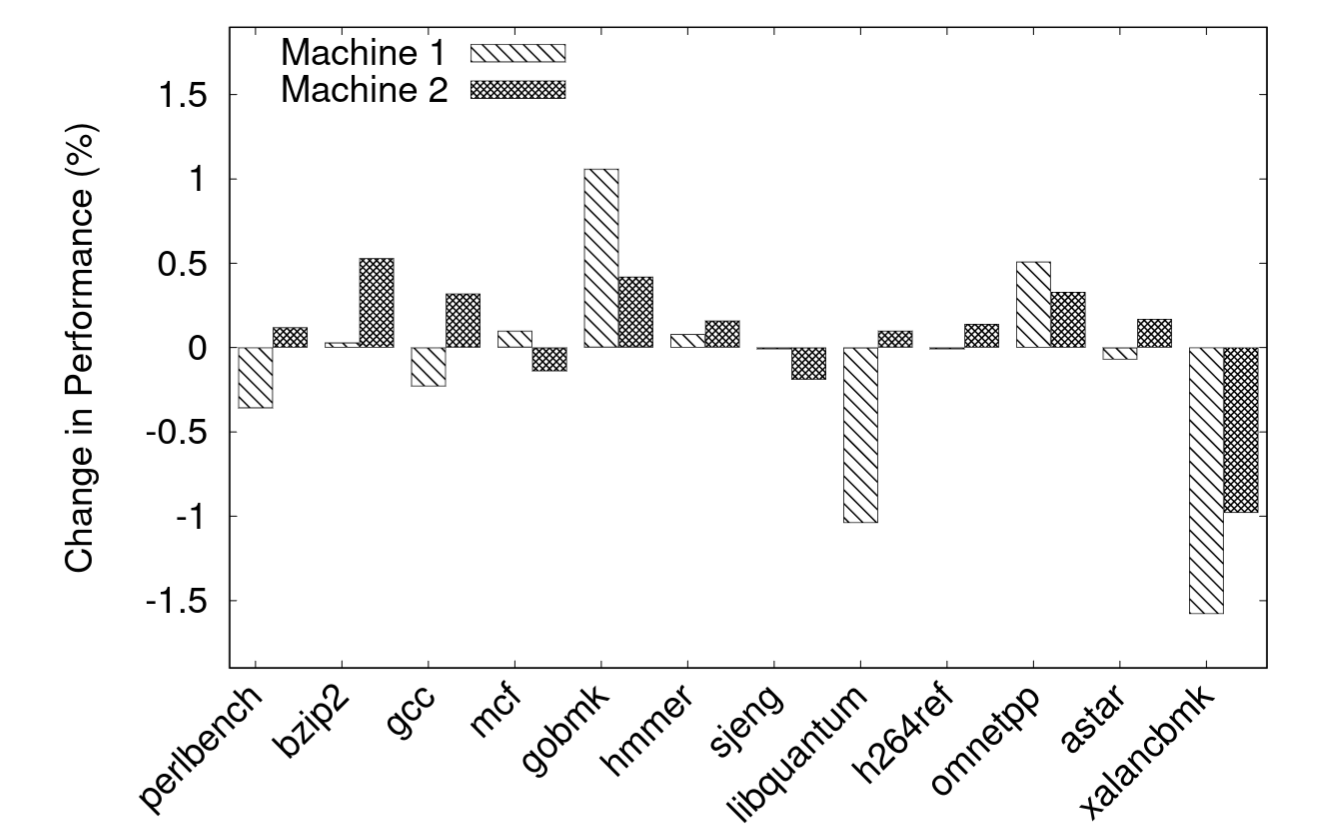
\includegraphics[width=\linewidth]{images/graph.png}
            \end{figure}
        \end{column}
    \end{columns}
    \pdfpcnote{
Object size is essentially unchanged at ±0.5\%. Runtime performance fluctuates
within ±1.6\%, within measurement noise. The key statistic: freeze instructions
represent only 0.04–0.06\% of all IR instructions — the new instruction is rarely
emitted, confirming the low practical overhead. Use the bar chart to ground the
claims visually.
}
\end{frame}


%%══════════════════════════════════════════════════════════════
%% CONCLUSION
%%══════════════════════════════════════════════════════════════
\begin{frame}[fragile]{Conclusion}
\begin{columns}[c]
    \begin{column}{0.50\textwidth}
    \begin{itemize}
        \item Undefined behaviour in compiler IR \textbf{enables} desirable optimizations
        \item Having \textbf{two distinct} semantics for deferred UB was a source of historical bugs
        \item The \texttt{freeze} instruction is now part of LLVM, so \texttt{undef} is now \textbf{deprecated}
    \end{itemize}
    \end{column}
    \begin{column}{0.54\textwidth}
        \begin{figure}
            \centering
            
\includegraphics[width=1.05\textwidth]{images/dragon-knight.png}
        \end{figure}
    \end{column}
\end{columns}

\pdfpcnote{
Close with the three takeaways: 

1. UB is necessary for desirable optimizations
2. Having two distinct deferred-UB mechanisms was a historic source of bugs
3. The freeze instruction is the clean solution now adopted by LLVM with undef deprecated. 
Leave time for questions — likely topics are the undef/poison distinction, why phi and
select are exceptions to poison propagation, and why freeze cannot be duplicated
or sunk into loops.
}

\end{frame}


%%══════════════════════════════════════════════════════════════
%% THANKS FOR YOUR ATTENTION
%%══════════════════════════════════════════════════════════════
\begin{frame}[plain, noframenumbering, label=thankyou]
  \begin{tikzpicture}[overlay, remember picture]
    \fill[UnipiBlue]
      ([yshift=-0.42\paperheight] current page.north east) --
      (current page.south east) --
      ([yshift=0.08\paperheight] current page.south west) --
      cycle;
    \node[anchor=south east, inner sep=0pt, draw=none,
          xshift=-0.018\paperheight, yshift=0.02\paperheight]
      at (current page.south east)
      {\pgfuseimage{logo}};
  \end{tikzpicture}
 

  %--- Main title ---%
  \vfill
  \begin{center}
    {\rmfamily\mdseries\fontsize{36}{42}\selectfont\color{BerkeleyBlueText}
      Thanks for your attention}
 
    \vspace{0.05cm}
    {\color{UnipiBlue!50}\rule{0.5\textwidth}{0.5pt}}
    \vspace{0.6cm}
 
    %{\large\color{BerkeleyBlueText} Subtext}
  \end{center}
  \vfill
 
\end{frame}


\end{document}
